\documentclass{beamer}

\mode<presentation> {
\usecolortheme{seagull}

\setbeamertemplate{footline}[page number]}
\usepackage{graphicx} 
\usepackage{booktabs} 
\usepackage{url}
\usepackage{hyperref}
\usepackage{listings}

\AtBeginSection[]{
  \begin{frame}
  \vfill
  \centering
    \usebeamerfont{title}\Huge{\insertsectionhead\par}
  \vfill
  \end{frame}
}

%-------------------------------------------------------------------------

\title[TLKDCC Power management]{Power management}
\author{Hans Holmberg}
\institute[LKTP]
{
Linux Kernel Teaching Project \\ 
\medskip
\textit{hans.holmberg@gmail.com}
}
\date{\today}
%------------------------------------------------------------------------
\begin{document}

\begin{frame}
\titlepage

\includegraphics{../common/tux} 
\end{frame}

\begin{frame}
\frametitle{Overview}
\tableofcontents 
\end{frame}

%-----------------------------------------------------------------------
\section{Overview}

\begin{frame}
\frametitle{Why bother with power management?}
\begin{itemize}
\item Cost of energy
\item Cost of cooling
\item Battery time
\item Skin temperature, CPU temperature restrictions
\end{itemize}
\end{frame}

\begin{frame}
\frametitle{Dynamic power dissapation}

Dynamic power dissaption (P), depends on capacitance(C), voltage(V) and and clock frequency (f):
\[P = CV^2f\]
\begin{itemize}
	\item Capacitance is a constant in a given system and depends on the number of gates
	\item Minimal voltage depends on clock frequency, higher voltage is needed to charge capacitors as the frequency increases
	\item Performance scales with frequency
\end{itemize}
\end{frame}

\begin{frame}
\frametitle{Leakage}
\begin{itemize}
	\item Even when the clock frequency is reduced to zero, the IP block will consume power due to leakage.
	\item To remove the leakage power consumtion, the voltage needs to be gated(turned off).
	\item Gating power comes at a cost: the internal state needs to be reinitialized when the block is power up again.
\end{itemize}
\end{frame}

\begin{frame}
\frametitle{So what can we do?}
\begin{itemize}
	\item Scale down clock frequencies (while maintaining reasonable performance)
	\item Utilize any ip-block specific powersave functions
	\item Power down unused parts of the system
	\item Put the whole system to sleep when acceptable
\end{itemize}
\end{frame}
%-----------------------------------------------------------------------
\section{System / static power management}
\begin{frame}
\frametitle{Suspend}
\begin{itemize}
	\item Initiated by userspace (i.e. after inactivity)
	\begin{itemize}
		\item \textbf{echo mem \textgreater /sys/power/state}
	\end{itemize}
	\item Puts the whole system to sleep
	\item Userspace is frozen
	\item Big latency cost
\end{itemize}
\begin{center}

\includegraphics[width=6cm]{media/tuxsleep.png}
\end{center}
\end{frame}

\begin{frame}
\frametitle{Suspend-resume cycle}
\begin{enumerate}
	\item Freeze tasks
	\item Suspend devices
	\item Disable nonboot cpus
	\item Enter suspend
	\item - wakeup event - 
	\item Enable nonboot cpus
	\item Resume devices
	\item Thaw tasks
\end{enumerate}
\end{frame}

\begin{frame}
\frametitle{Driver hooks}
\begin{enumerate}
	\item \textbf{prepare}: stop registring new devices
	\item \textbf{suspend}: stop IO, put device in low power state
	\item \textbf{suspend\_late}: save device state (if not done yet)
	\item \textbf{suspend\_noirq}: save device state if irqs need to be off
\noindent\rule{4cm}{0.4pt}
	\item \textbf{resume\_noirq}: undo suspend\_noirq
	\item \textbf{resume\_early}: undo suspend\_late
	\item \textbf{resume}: undo suspend
	\item \textbf{complete}: undo prepare
\end{enumerate}
See the kernel docs for details \footnote{\url{https://www.kernel.org/doc/Documentation/power/devices.txt}}
\end{frame}

\begin{frame}
\frametitle{Example - lpc32xx touchscreen driver}
\begin{itemize}
	\item The lpc32xx driver implements suspend and resume
	\item drivers/input/touchscreen/lpc32xx\_ts.c:377
\end{itemize}
\end{frame}


\begin{frame}
\frametitle{Power Management Domains}
\begin{itemize}
	\item Normally, the driver's bus framework calls the suspend hooks
	\item device.dev\_pm\_domain can be used to override the normal callbacks
	\item Used if power states needs to be coordinated across devices sharing a power resource (clocks, power planes, ..)
\end{itemize}
\end{frame}

\begin{frame}
\frametitle{Different policies}
\begin{itemize}
	\item PCs: suspend on inactivity 
	\item Handheld devices: suspend as soon as possible (opportunistic)
	\item Opportunistic suspend configured via /sys/power/autosleep
\end{itemize}
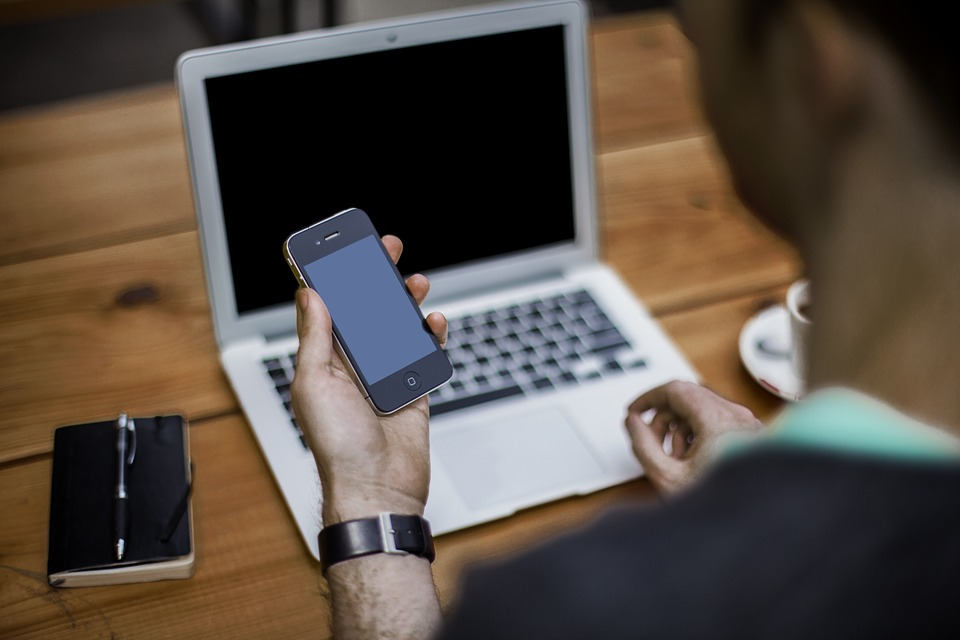
\includegraphics[width=6cm]{media/pchandheld.jpg}
\end{frame}

\begin{frame}
\frametitle{Wake locks and wakeup sources}
\begin{itemize}
	\item For opportunistic suspend, userspace and drivers needs to be able to keep the system awake if needed be
	\item Drivers can grab a wake lock to block suspend
	\item Userspace can create and unlock locks via
	\begin{itemize}
		\item /sys/power/wake\_lock 
		\item /sys/power/wake\_unlock
	\end{itemize}
	\item Statistics on wakelocks are available in /sys/kernel/debug/wakeup\_sources
\end{itemize}
\end{frame}

%-----------------------------------------------------------------------
\section{Runtime power management}

\begin{frame}
\frametitle{Runtime/dynamic power management}

\begin{itemize}
	\item Put devices in low-power mode when possible
	\item Userspace should not be affected
\end{itemize}
\begin{center}
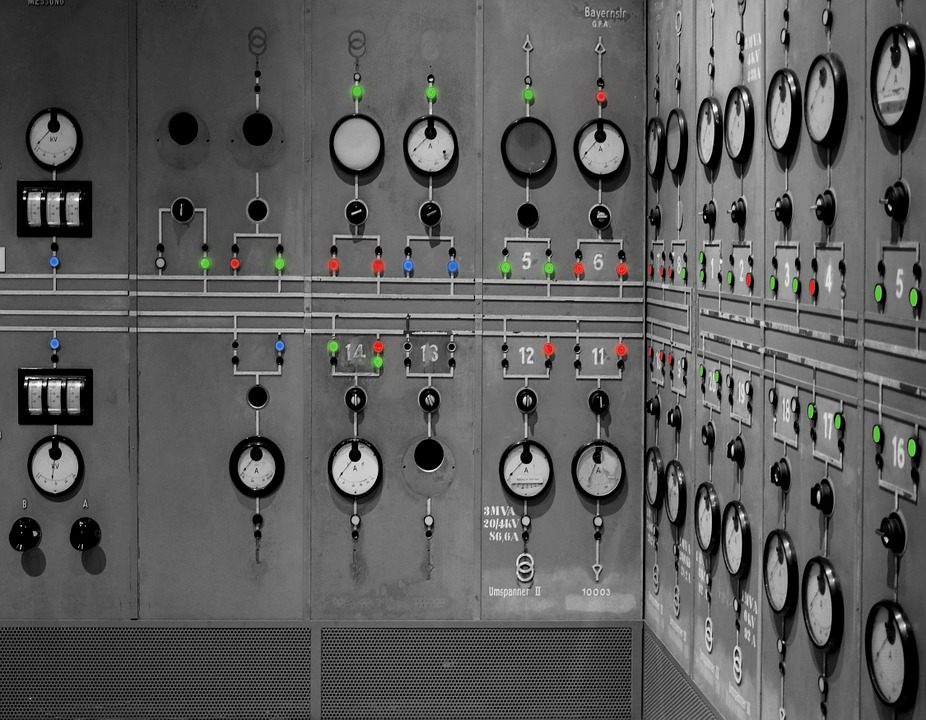
\includegraphics[width=6cm]{media/powerswitches.jpg}
\end{center}
\end{frame}


\begin{frame}
\frametitle{The runtime PM core}
\begin{itemize}
	\item Drivers inform the PM core when a device is in use via:
	\begin{itemize}
		\item pm\_runtime\_get (I'm about to use it)
		\item pm\_runtime\_put (Done for now)
	\end{itemize}
	\item The PM core counts uses and triggers driver callbacks:
	\begin{itemize}
		\item runtime\_suspend (use count 1 -\textgreater 0)
		\item runtime\_resume (use count 0 -\textgreater 1)
	\end{itemize}
	\item It is also possible to suspend automatically after a specified inactivity time (autosuspend)
	\item API details in the kernel docs \footnote{\url{https://www.kernel.org/doc/Documentation/power/runtime\_pm.txt}}
\end{itemize}
\end{frame}

\begin{frame}
\frametitle{Combining system and runtime PM}
Differences:
\begin{itemize}
	\item System PM: suspend when requested, resume with system
	\item Runtime PM: suspend on inactivity, resume when needed
\end{itemize}
Solution:
\begin{itemize}
	\item Implement runtime PM first
	\item If needed, implement system pm as well, and try to reuse runtime pm callbacks when possible
\end{itemize} 
See Kevin Hilman's presentation for more details \footnote{\url{http://www.slideshare.net/linaroorg/runtime-pm}}
\end{frame}

\begin{frame}
\frametitle{CPU Power save in idle}
\begin{center}

\includegraphics[width=3cm]{media/catnap.jpg}
\end{center}
\begin{itemize}
	\item When the CPU is not executing a task, Linux will try to put the processor in a low-power idle mode
	\item The idle mode is selected by a cpuidle governor that tries to balance power with wake-up latency depending on cpu-utilization
	\item Idle modes are architecture specific 
\end{itemize}
\end{frame}

%-----------------------------------------------------------------------
\section{Frequency and voltage scaling}

\begin{frame}
\frametitle{Frequency and voltage scaling}
\begin{itemize}
\item Governors together with cpufreq drivers can control the performance and power consumtion according to different policies
\item Cpufreq drivers provides architecture-specific implementation
\item Governors provide generic policies
\item Choosing governor is up to the user
\end{itemize}

\includegraphics[width=3cm]{media/tuxpolitician.png}
\end{frame}

\begin{frame}
\frametitle{Governors 1/2}
\begin{itemize}
\item \textbf{Performance}: sets the CPU statically to the
highest frequency within the borders of scaling\_min\_freq and
scaling\_max\_freq.

\item \textbf{Powersave}: sets the CPU statically to the
lowest frequency within the borders of scaling\_min\_freq and
scaling\_max\_freq.

\item \textbf{Userspace}: allows the user, or any userspace
program running with UID "root", to set the CPU to a specific frequency
by making a sysfs file "scaling\_setspeed" available in the CPU-device
directory.

\end{itemize}
\end{frame}

\begin{frame}
\frametitle{Governors 2/2}
\begin{itemize}

\item \textbf{Ondemand}: sets the CPU depending on the
current usage. To do this the CPU must have the capability to
switch the frequency very quickly.

\item \textbf{Conservative}:  much like the "ondemand" governor, sets the CPU depending on the current usage. Gracefully increases and decreases the CPU speed
rather than jumping to max speed the moment there is any load on the
CPU. 
\end{itemize}
\end{frame}


%-----------------------------------------------------------------------
\begin{frame}
\Huge{\centerline{Thanks!}}
\end{frame}

\end{document} 
